\documentclass[a4page]{article}
\usepackage[14pt]{extsizes} % для того чтобы задать нестандартный 14-ый размер шрифта
\usepackage[utf8]{inputenc}
\usepackage[T1, T2A]{fontenc}
\usepackage[utf8]{inputenc}
\usepackage[russian]{babel} % поддержка русского языка
\usepackage{amsmath}  %  математические символы
\usepackage[left=25mm, top=20mm, right=15mm, bottom=30mm, footskip=15mm]{geometry} % настройки полей документа
\usepackage{indentfirst} % по умалчанию убирается отступ у первого абзаца в секции, это отменяет это.
\usepackage{paralist} % добавить компактные списки (compactitem, compactenum, compactdesc)

\usepackage{fancyvrb}
\usepackage{fancyref}
\usepackage{framed}
\usepackage{url}
\usepackage{csquotes}
\usepackage{listings}

\usepackage{graphicx}
\graphicspath{ {./Images/} }

\usepackage{float}
\floatstyle{ruled}

\usepackage[
	backend=biber,
	sorting=nyt,
	bibstyle=gost-numeric,
	citestyle=gost-numeric
]{biblatex}

\usepackage[
	bookmarks=true, colorlinks=true, unicode=true,
	urlcolor=black,linkcolor=black, anchorcolor=black,
	citecolor=black, menucolor=black, filecolor=black,
]{hyperref}

\addbibresource{sources.bib}

\renewcommand{\baselinestretch}{1.25}

\begin{document}

\begin{titlepage}
	\begin{center}
		\hfill \break
		\textbf{
			\large{РОССИЙСКИЙ УНИВЕРСИТЕТ ДРУЖБЫ НАРОДОВ}\\
			\normalsize{Факультет физико-математических и естественных наук}\\
			\normalsize{Кафедра прикладной информатики и теории вероятностей}\\
		}
		\vspace*{\fill}
		\Large{\textbf{Архитектура REST взаимодействия компонентов распределенного приложения в сети.\\Обозначение объектов JavaScript (JSON).}}
		\\
		\underline{\textit{\normalsize{Дисциплина: Вычислительные системы, сети и телекоммуникации}}}
		\vspace*{\fill}

	\end{center}

	\begin{flushright}
		Студент: \underline{Матюхин Григорий}\\ \vspace{0.5cm}
		Группа: \underline{НПИбд-01-21}
	\end{flushright}

	\begin{center} \textbf{МОСКВА} \\ 2023 г. \end{center}
	\thispagestyle{empty}

\end{titlepage}

\newpage

\tableofcontents

\newpage
\section{Введение}
Архитектура программной системы --- это метафора, аналогичная архитектуре здания.
Она функционирует как чертежи системы и проекта разработки,
которые впоследствии могут быть использовано для экстраполяции задач,
необходимых для выполнения вовлеченными командами и людьми.
Архитектурный стиль REST является де-факто стандартом для создания веб-сервисов в интернете,
потому что их легко создавать и легко использовать.

В данном реферате описываются основы этой архитектуры, возможности, примеры ее использования,
а также использование текстового формата JSON вместе с REST.

\newpage
\section{REST}
REST (от англ. Representational State Transfer ---
<<передача репрезентативного состояния>> или <<передача "самоописываемого" состояния>>) ---
архитектурный стиль взаимодействия компонентов распределенного приложения в сети~\cite{REST}.
Другими словами, REST --- это набор правил того,
как программисту организовать написание кода серверного приложения,
чтобы все системы легко обменивались данными и приложение можно было масштабировать.
REST представляет собой согласованный набор ограничений,
учитываемых при проектировании распределенной гипермедиа-системы.

Для веб-служб, построенных с учетом REST (то есть не нарушающих накладываемых им ограничений),
применяют термин <<RESTful>>.

\subsection{Свойства архитектуры REST}
Архитектурный стиль REST разработан для сетевых приложений,
в частности для клиент-серверных приложений.
Но более того, он предназначен для использования в масштабах интернета,
поэтому связь между пользовательским агентом (клиентом) и
исходным сервером должна быть как можно более свободной,
чтобы способствовать широкомасштабному внедрению.

Сильное разделение клиента и сервера вместе с текстовой передачей информации
с использованием единого протокола адресации послужило основой для удовлетворения требований интернета:
надежность, независимость развертывания компонентов,
крупнозернистая передача данных и низкий входной барьер для потребителей и
производителей контента и разработчиков.

Ограничения архитектурного стиля REST влияют на следующие архитектурные свойства:

\begin{itemize}
	\item производительность при взаимодействии компонентов,
	      которая может быть доминирующим фактором воспринимаемой
	      пользователем производительности и эффективности сети;
	\item масштабируемость, позволяющая поддерживать большое количество компонентов
	      и взаимодействие между компонентами;
	\item простота единого интерфейса;
	\item модифицируемость компонентов для удовлетворения меняющихся потребностей
	      (даже во время работы приложения);
	\item видимость связи между компонентами сервисными агентами;
	\item переносимость компонентов за счет перемещения программного кода вместе с данными;
	\item надежность в устойчивости к сбоям на системном уровне при наличии сбоев в компонентах,
	      соединителях или данных.
\end{itemize}

\subsection{Требования к архитектуре REST}
Существует шесть обязательных ограничений для построения распределенных REST-приложений~\cite{RESTful}.
Накладываемые ограничения определяют то как сервер может обрабатывать и отвечать на запросы клиентов.
Действуя в рамках этих ограничений,
система приобретает такие желательные свойства как производительность,
масштабируемость, простоту, способность к изменениям, переносимость, отслеживаемость и надежность.

\subsubsection{Модель клиент-сервер}
Модель клиент-сервер отделяет задачи пользовательского интерфейса от задач хранения данных.
Таким образом, повышается переносимость пользовательского интерфейса.
В случае с интернетом для большинства платформ разработано множество веб-браузеров
без необходимости знания каких-либо серверных реализаций.
Разделение также упрощает серверные компоненты, улучшая масштабируемость,
но, что более важно, оно позволяет компонентам развиваться независимо,
что необходимо в мастштабах интернета.

\subsubsection{Отсутствие состояния}
Протокол взаимодействия между клиентом и сервером требует соблюдения следующего условия:
в период между запросами клиента никакая информация о состоянии клиента на сервере не хранится
(Stateless protocol или <<протокол без сохранения состояния>>).
Все запросы от клиента должны быть составлены так,
чтобы сервер получил всю необходимую информацию для выполнения запроса.
Состояние сессии при этом сохраняется на стороне клиента.
Информация о состоянии сессии может быть передана сервером какому-либо другому сервису
(например, в службу базы данных) для поддержания устойчивого состояния,
например, на период установления аутентификации.
Клиент инициирует отправку запросов, когда возникает необходимость перейти в новое состояние.

\subsubsection{Кэширование}
Как и во всемирной паутине, клиенты и посредники могут кэшировать ответы.
Ответы должны явно или неявно определять себя как кэшируемые или некэшируемые,
чтобы клиенты не предоставляли устаревшие или неподходящие данные в ответ на дальнейшие запросы.
Хорошо управляемое кэширование частично или полностью устраняет некоторые взаимодействия
между клиентом и сервером, дополнительно повышая масштабируемость и производительность.
Кэширование может выполняться на клиентской машине в памяти или в хранилище кеша браузера.
Кроме того, кэш может храниться в сети доставки контента (CDN).

\subsubsection{Единообразие интерфейса}
Ограничение единого интерфейса имеет основополагающее значение для проектирования любой RESTful системы.
Это упрощает и разделяет архитектуру, что позволяет каждой части развиваться независимо.
Четыре ограничения для единообразного интерфейса:

\begin{itemize}
	\item Идентификация ресурсов в запросах.
	      Отдельные ресурсы идентифицируются в запросах, например, с помощью URI в веб-службах.
	      Сами ресурсы концептуально отделены от представлений, возвращаемых клиенту.
	      Например, сервер может отправлять данные из своей базы данных в формате HTML,
	      XML или JSON, ни один из которых не является внутренним представлением данных.
	\item Манипулирование ресурсами с помощью представлений.
	      Когда клиент содержит представление ресурса, включая любые прикрепленные метаданные,
	      у него достаточно информации для изменения или удаления состояния ресурса.
	\item <<Самоописываемые>> сообщения.
	      Каждое сообщение содержит достаточно информации, чтобы описать, как его обрабатывать.
	      Например, какой синтаксический анализатор вызывать,
	      можно определить по заголовку \texttt{content-type}.
	\item Гипермедиа как механизм состояния приложения (HATEOAS).
	      Получив доступ к начальному URI для приложения REST --- аналогично тому,
	      как пользователь получает доступ к домашней странице веб-сайта, ---
	      клиент REST должен иметь возможность динамически использовать предоставленные сервером ссылки
	      для обнаружения всех доступных ресурсов, в которых он нуждается.
	      Клиенту также нет необходимости запоминать структуру сервера,
	      если все необходимые данные можно получить по ссылкам (подробнее см. секцию \ref{hateoas}).
\end{itemize}

\subsubsection{Слои}
Клиент обычно не способен точно определить,
подключен ли он напрямую к конечному серверу или к промежуточному узлу.
Если между клиентом и сервером размещен прокси-сервер или балансировщик нагрузки,
это не повлияет на их связь, и не потребуется обновлять код клиента или сервера.
Промежуточные серверы могут улучшить масштабируемость системы,
обеспечивая балансировку нагрузки и общие кэши.
Кроме того, безопасность можно добавить как уровень поверх веб-сервисов,
отделив бизнес-логику от логики безопасности.
Добавление безопасности в качестве отдельного уровня обеспечивает соблюдение политик безопасности.
Наконец, промежуточные серверы могут вызывать несколько других серверов, чтобы сгенерировать ответ клиенту.

\subsubsection{Код по требованию}
REST может позволить расширить функциональность клиента за счет загрузки кода с сервера
в виде апплетов или скриптов.

\subsection{HATEOAS}\label{hateoas}
Гипермедиа как механизм состояния приложения (HATEOAS) --- это ограничение архитектуры приложений REST,
которое отличает ее от других архитектур сетевых приложений.
С HATEOAS клиент взаимодействует с сетевым приложением,
чьи серверы приложений динамически предоставляют информацию через гипермедиа.
Клиенту REST практически не нужны предварительные знания о том,
как взаимодействовать с приложением или сервером, помимо общего понимания гипермедиа.
Ограничения, налагаемые HATEOAS, разделяют клиент и сервер.
Это позволяет функциональности сервера развиваться независимо~\cite{rest-of-rest}.

\subsubsection{Пример}
Пользовательский агент отправляет HTTP-запрос к REST API через URL-адрес точки входа.
Все последующие запросы, которые может сделать клиент, обнаруживаются внутри ответа на каждый запрос.
Типы мультимедиа, используемые для этих представлений, и отношения ссылок, которые они могут содержать,
являются частью API. Клиент переходит через состояния приложения,
выбирая из ссылок в представлении или манипулируя представлением другими способами,
предоставляемыми его типом носителя.
Таким образом RESTful-взаимодействия работают через гипермедиа,
а не через заранее указанный интерфейс~\cite{REST-hyper}.

Например, этот GET запрос извлекает ресурс учетной записи,
запрашивая детали в представлении XML~\cite{hateoas}:

\begin{lstlisting}
GET /accounts/12345 HTTP/1.1
Host: bank.example.com
Accept: application/xml
...
\end{lstlisting}

Ответ:

\begin{lstlisting}
HTTP/1.1 200 OK
<?xml version="1.0"?>
<account>
    <account_number>12345</account_number>
    <balance currency="usd">100.00</balance>
    <link rel="deposit" href="/account/12345/deposit" />
    <link rel="withdraw" href="/account/12345/withdraw" />
    <link rel="transfer" href="/account/12345/transfer" />
    <link rel="close" href="/account/12345/close" />
</account>
\end{lstlisting}

Ответ содержит следующие возможные последующие ссылки:
POST депозит, снятие средств, перевод или запрос на закрытие (закрыть учетную запись).

При отрицательном балансе, будет другой набор доступных ссылок.

\begin{lstlisting}
GET /account/12345 HTTP/1.1

HTTP/1.1 200 OK
<?xml version="1.0"?>
<account>
    <account_number>12345</account_number>
    <balance currency="usd">-25.00</balance>
    <link rel="deposit" href="/account/12345/deposit" />
</account>
\end{lstlisting}

Сейчас доступна только одна ссылка: внести больше денег
(путем POST запроса на \texttt{/accounts/12345/deposits}).
В текущем состоянии другие ссылки недоступны.
Отсюда и термин <<механизм состояния приложения>> --- возможные действия зависят от состояния ресурса.

Клиенту не нужно понимать каждый тип мультимедиа и механизм связи, предлагаемый сервером.
Способность понимать новые типы мультимедиа может быть получена во время выполнения
с помощью <<кода по запросу>>, предоставляемого сервером.

\subsection{Преимущества}
Рой Филдинг указывал, что приложения, не соответствующие приведенным условиям,
не могут называться REST-приложениями. Если же все условия соблюдены, то, по его мнению,
приложение получит следующие преимущества~\cite{REST}:

\begin{itemize}
	\item Надежность (за счет отсутствия необходимости сохранять информацию о состоянии клиента,
	      которая может быть утеряна);
	\item Производительность (за счет использования кэша);
	\item Масштабируемость;
	\item Прозрачность системы взаимодействия (особенно необходимая для приложений обслуживания сети);
	\item Простота интерфейсов;
	\item Портативность компонентов;
	\item Легкость внесения изменений;
	\item Способность эволюционировать, приспосабливаясь к новым требованиям (на примере Всемирной паутины).
\end{itemize}

\newpage
\section{JSON}
JSON (англ. JavaScript Object Notation) ---
текстовый формат обмена данными, основанный на JavaScript~\cite{rfc8259}~\cite{ISO21778}.
Как и многие другие текстовые форматы, JSON легко читается людьми.
Формат JSON был разработан Дугласом Крокфордом.

Несмотря на происхождение от JavaScript
(точнее, от подмножества языка стандарта ECMA-262 1999 года~\cite{ecma:262}),
формат считается независимым от языка и может использоваться практически с любым языком программирования.
Для многих языков существует готовый код для создания и обработки данных в формате JSON.

\subsection{Синтаксис}
JSON построен на двух структурах~\cite{json}:

\begin{itemize}
	\item Коллекция пар имя/значение.
	      В различных языках это реализуется как объект, запись, структура, словарь, хеш-таблица,
	      список с ключами или ассоциативный массив.
	\item Упорядоченный список значений.
	      В большинстве языков это реализовано в виде массива, вектора, списка или последовательности.
\end{itemize}

Это универсальные структуры данных. Практически все современные языки программирования поддерживают их
в той или иной форме. Имеет смысл, чтобы формат данных, взаимозаменяемый с языками программирования,
также основывался на этих структурах.

В JSON они принимают следующие виды (см. \hyperref[appendix]{приложение А}):
\begin{itemize}
	\item \textit{Объект} представляет собой неупорядоченный набор пар имя/значение.
	      Объект начинается с $\{_{\textup{левой скобки}}$ и заканчивается $\}_{\textup{правой скобкой}}$.
	      За каждым именем следует $:_\textup{двоеточие}$, а пары имя/значение разделяются $,_\textup{запятой}$.
	\item \textit{Массив} --- это упорядоченный набор значений.
	      Массив начинается с $[_{\textup{левой скобки}}$ и заканчивается $]_{\textup{правой скобкой}}$.
	      Значения разделяются $,_\textup{запятой}$.
	\item \textit{Значение} может быть \textit{строкой} в двойных кавычках,
	      или \textit{числом}, или \texttt{true}, или \texttt{false}, или \texttt{null}, или \textit{объектом},
	      или \textit{массивом}. Эти структуры могут быть вложенными.
	\item \textit{Строка} --- это последовательность из нуля или более символов Юникода,
	      заключенная в двойные кавычки и использующая символы обратной косой черты.
	      Один символ представлен в виде строки из одного элемента.
	\item \textit{Число} очень похоже на число C или Java, за исключением того,
	      что восьмеричный и шестнадцатеричный форматы не используются.
	\item \textit{Пробелы} могут быть вставлены между любой парой токенов.
\end{itemize}

За исключением нескольких деталей кодировки, это полностью описывает язык.

\subsection{Расширения в RESTful архитектуре}

\subsubsection{HAL}
Hypertext Application Language (HAL, Язык Гипертекстовых Приложений) ---
это разрабатываемый (Internet Draft, или ID) стандарт для определения гипермедиа,
таких как ссылки на внешние ресурсы в форматах JSON или XML~\cite{hal}.

HAL структурирован таким образом, чтобы представлять элементы на основе двух концепций: ресурсы и связи.
Ресурсы состоят из ссылок URI ресурсов внедренных в стандартные форматы данных
(будь то JSON или XML) а не ссылок URI. Ссылки имеют целевой URI, имя (называемый 'rel'),
а также дополнительные свойства, предназначенные для учета устаревания и согласования содержимого.

\newpage
Пример:

\begin{lstlisting}
{
  "_links": {
    "self": {
      "href": "http://example.com/api/book/hal-cookbook"
    },
    "next": {
      "href": "http://example.com/api/book/hal-case-study"
    },
    "prev": {
      "href": "http://example.com/api/book/json-and-beyond"
    }
  },
  "_embedded": {
    "author": {
      "_links": {
        "self": {
          "href": "http://example.com/api/author/shahadat"
        }
      },
      "id": "shahadat",
      "name": "Shahadat Hossain Khan",
      "homepage": "http://author-example.com"
    }
  },
  "id": "hal-cookbook",
  "name": "HAL Cookbook"
}
\end{lstlisting}

\subsubsection{JSON-LD}
JSON-LD (<<JavaScript Object Notation for Linked Data>> ---
объектная нотация JavaScript для связанных данных) ---
один из методов передачи связанных данных с использованием текстового формата JSON~\cite{json-ld}.
Формат имеет целью упростить усилия разработчиков по преобразованию существующих JSON-данных в JSON-LD.
JSON-LD является рекомендацией W3C и разрабатывался Linking Data Community Group,
а затем --- RDF Working Group.

Следующий пример описывает человека (Person) в терминах онтологии из словаря FOAF.
\begin{lstlisting}
{
  "@context": {
    "name": "http://xmlns.com/foaf/0.1/name",
    "homepage": {
      "@id": "http://xmlns.com/foaf/0.1/workplaceHomepage",
      "@type": "@id"
    },
    "Person": "http://xmlns.com/foaf/0.1/Person"
  },
  "@id": "https://me.example.com",
  "@type": "Person",
  "name": "John Smith",
  "homepage": "https://www.example.com/"
}
\end{lstlisting}

Сначала JSON-свойства \texttt{name} и \texttt{homepage},
а также тип объекта \texttt{Person} связываются с терминами словаря FOAF,
затем значению свойства \texttt{homepage} назначается тип \texttt{@id}:
это означает, что значение свойства \texttt{@id}
(в данном примере «http://xmlns.com/foaf/0.1/workplaceHomepage»)
служит для поля \texttt{homepage} уникальным идентификатором (IRI) и определяет контекст,
в котором следует обрабатывать данные поля \texttt{homepage}.
Это позволяет однозначно описать в JSON-документе объект \texttt{Person},
основываясь на модели RDF, определив все поля в объекте при помощи IRI.
Использование работающих (resolvable) ссылок на типы данных в формате IRI
позволяет встраивать такие объекты в другие RDF-документы, которые содержат больше информации,
а также дает возможность клиентам получить новые данные, просто пройдя по таким ссылкам.

Поскольку все данные имеют семантические аннотации, RDF-парсер сможет определить,
что этот документ содержит информацию о человеке
(по свойству \texttt{@type} содержащему значение \texttt{Person}).
Помимо этого RDF-парсер понимает словарь FOAF и по этому словарю сможет определить,
какое свойство JSON-объекта содержит имя человека (\texttt{name})
а в каком хранится адрес его домашней страницы (\texttt{homepage}).

\newpage
\section{Заключение}
В заключение я хотел бы еще раз подчеркнуть распространенность архитектуры программного обеспечения REST
и RESTful веб-сервисов в интернете. В конце концов, все сводится к тому,
что архитектура REST позволяет легко создавать масштабируемые и надежные сервисы на десятилетия вперед.

\newpage
\addcontentsline{toc}{section}{Приложение А. Синтаксические диаграммы JSON}
\section*{Приложение А. Синтаксические диаграммы JSON} \label{appendix}
\begin{enumerate}
	\item Объект \\
	      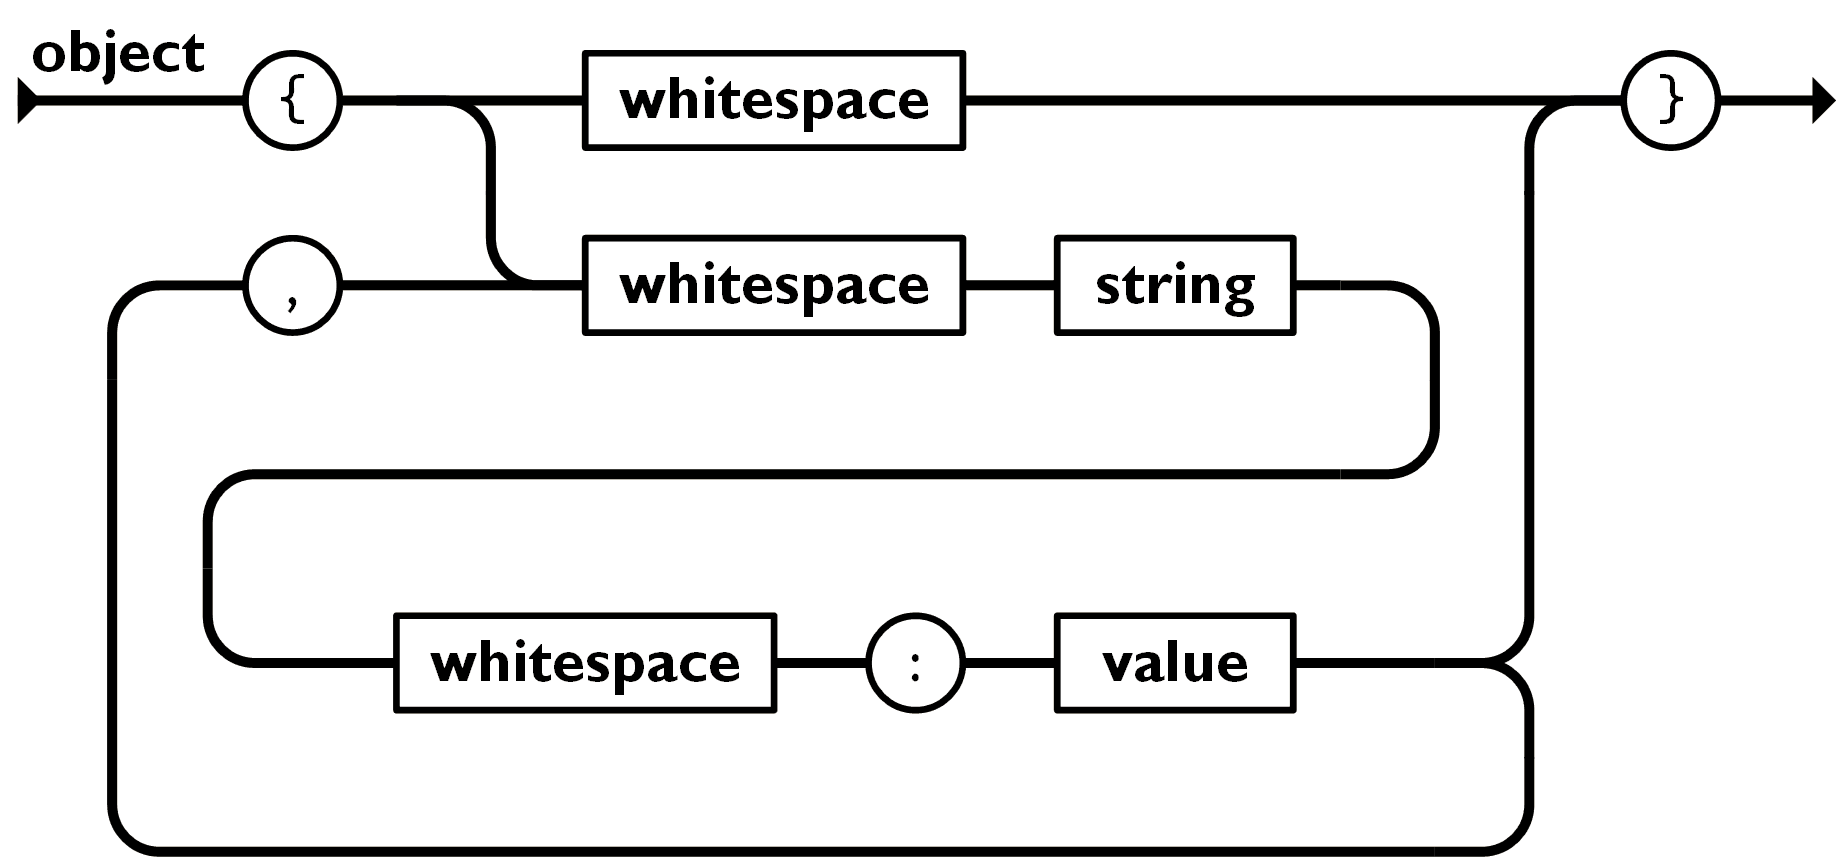
\includegraphics[scale=0.6]{object.png}
	\item Массив \\
	      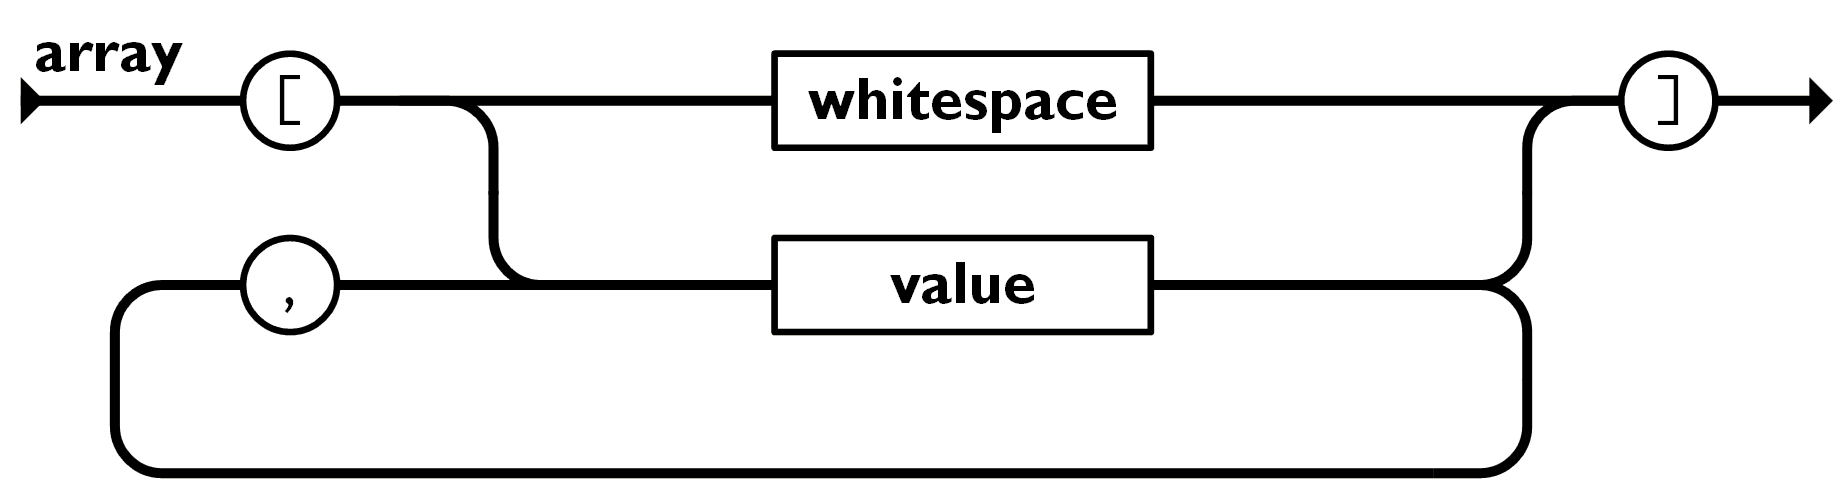
\includegraphics[scale=0.6]{array.png}
	\item Значение \\
	      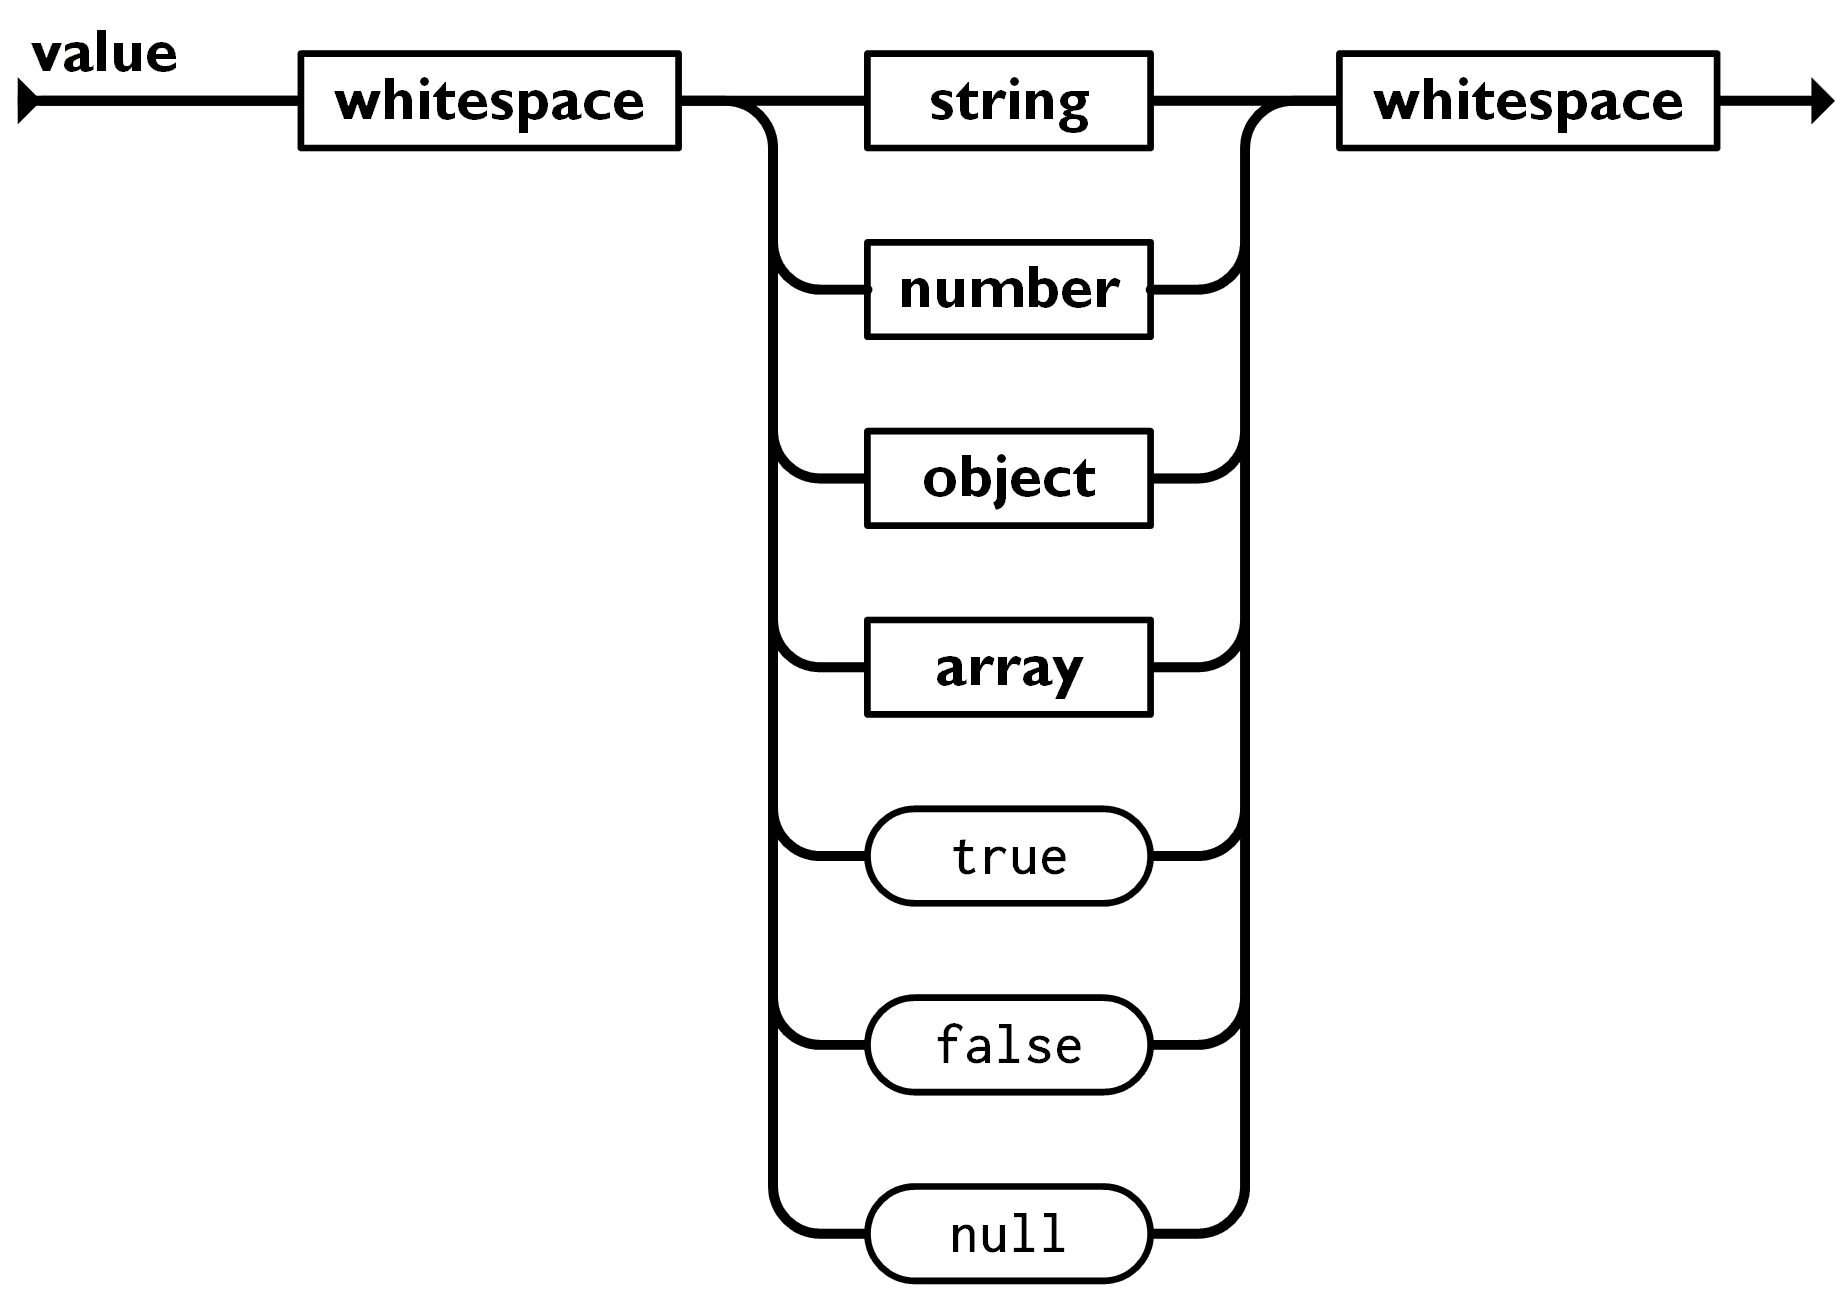
\includegraphics[scale=0.6]{value.png}
	      \newpage
	\item Строка \\
	      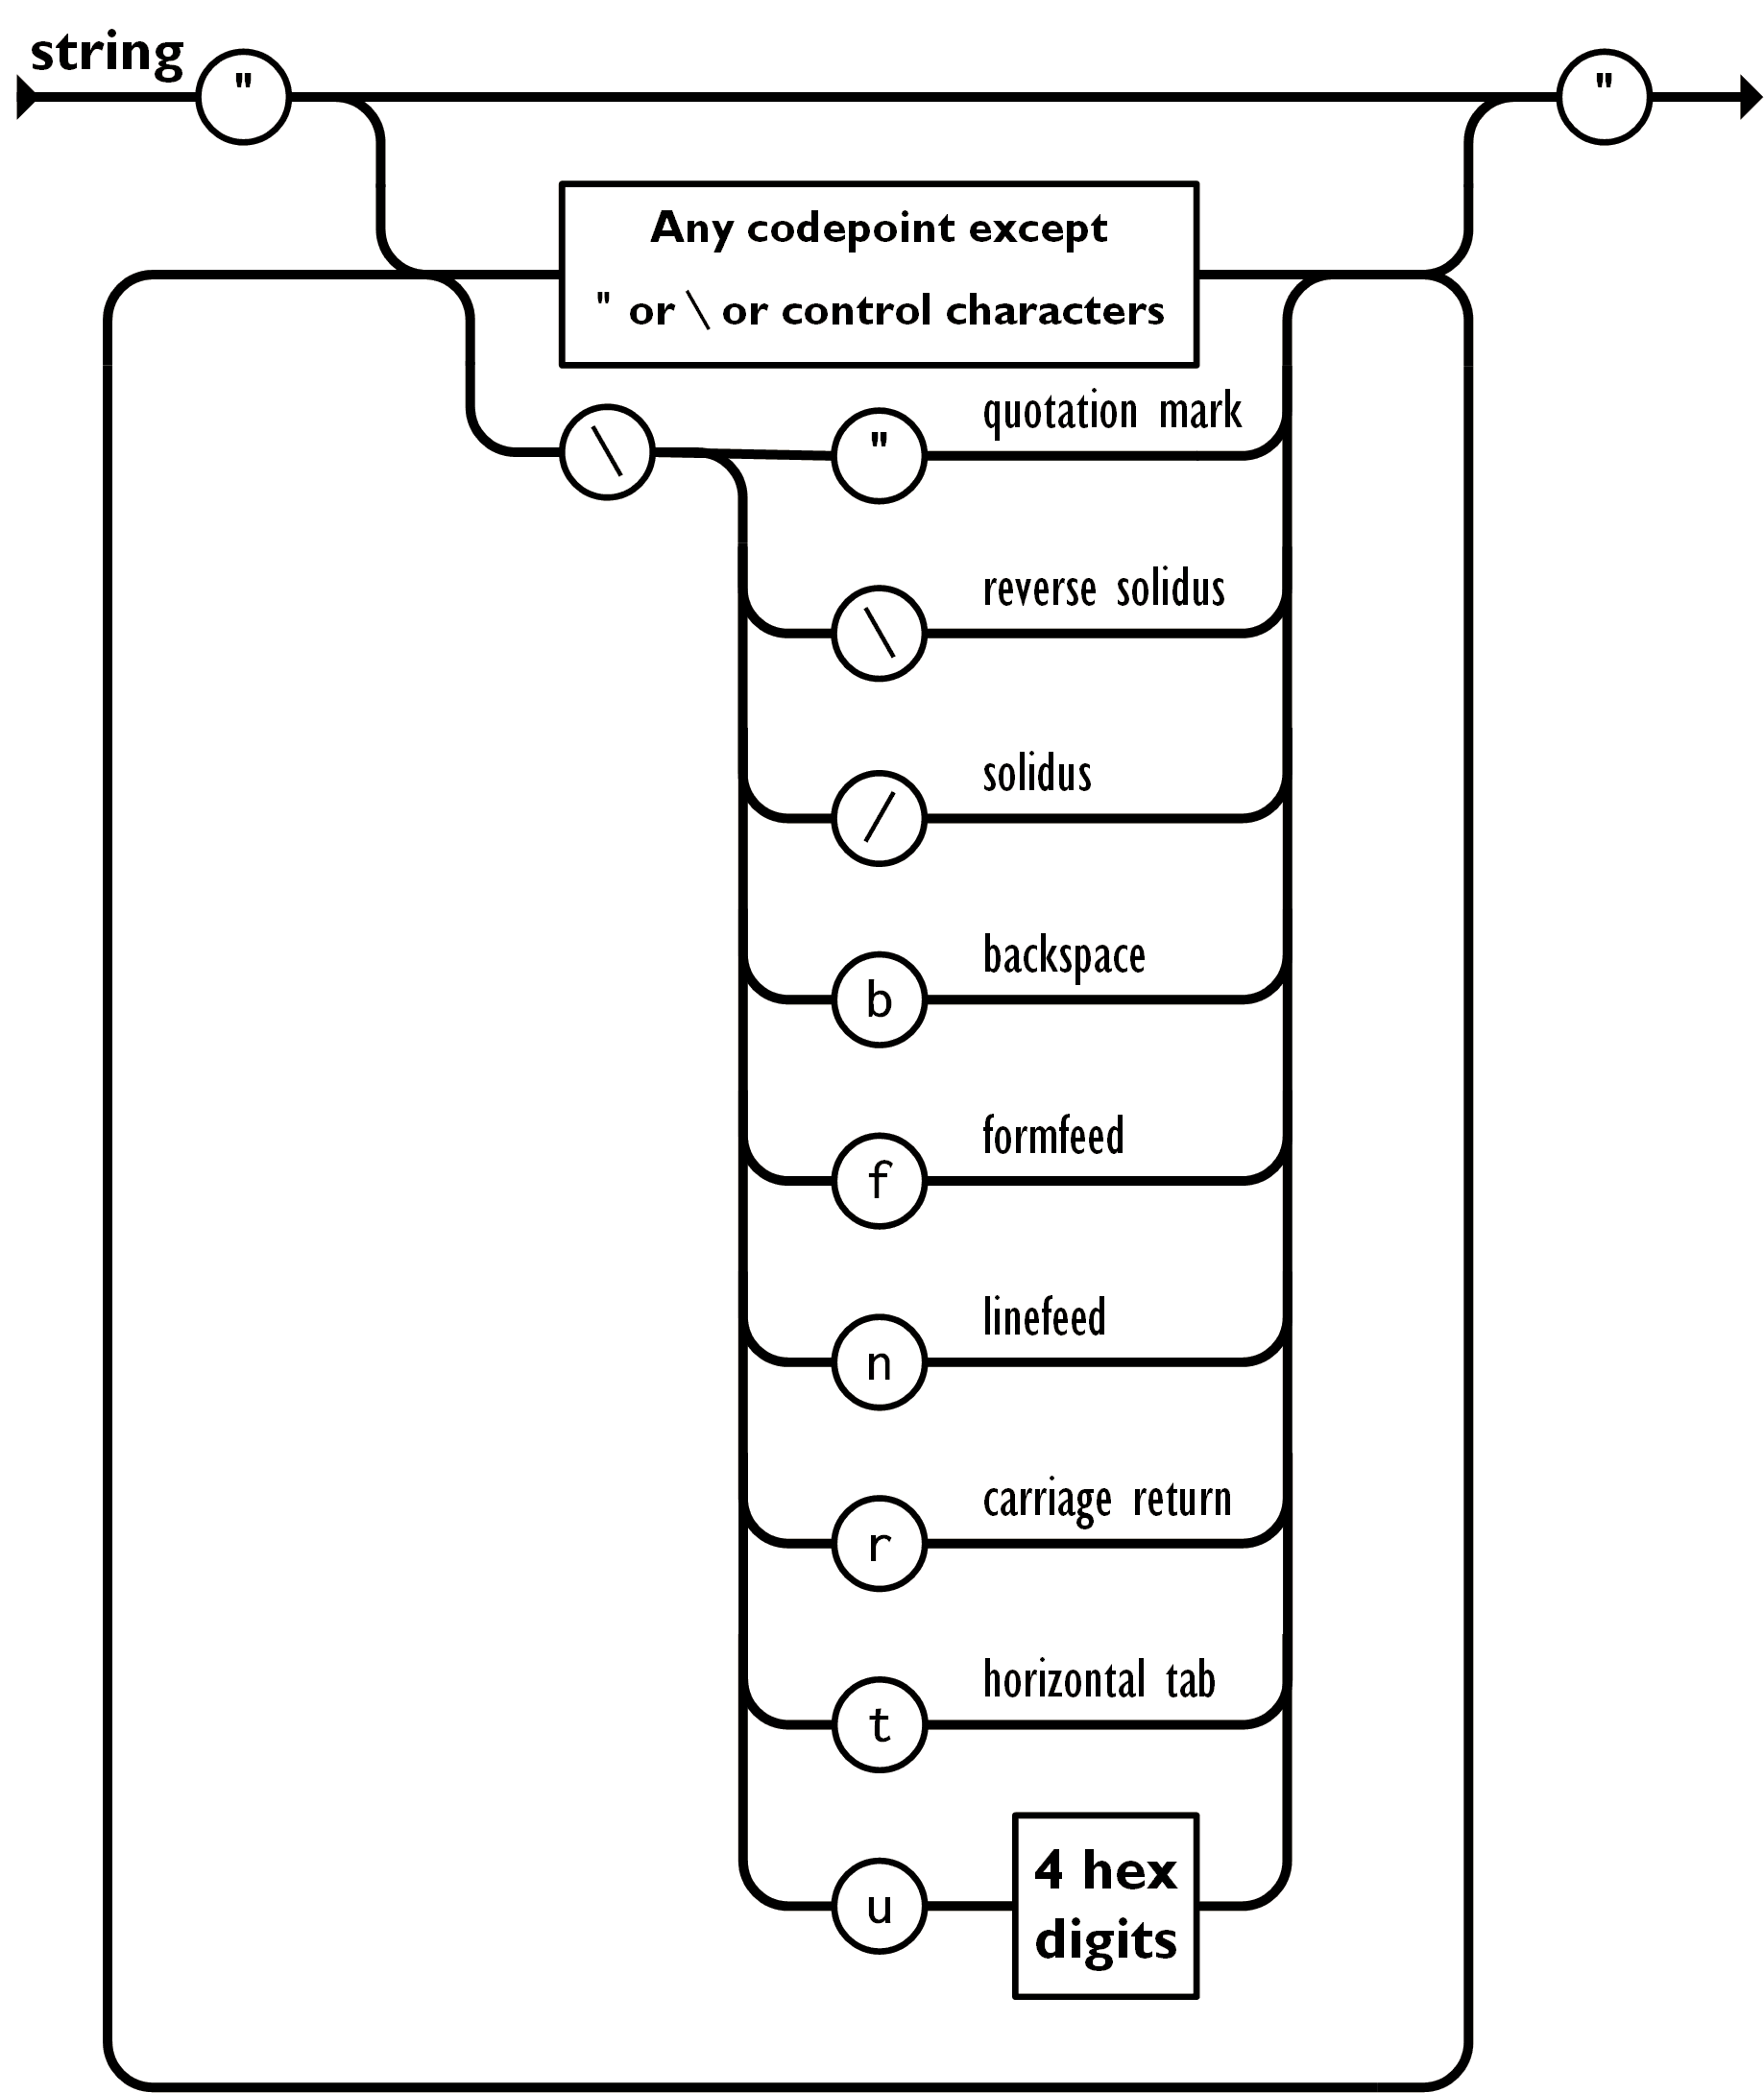
\includegraphics[scale=0.6]{string.png}
	      \newpage
	\item Объект \\
	      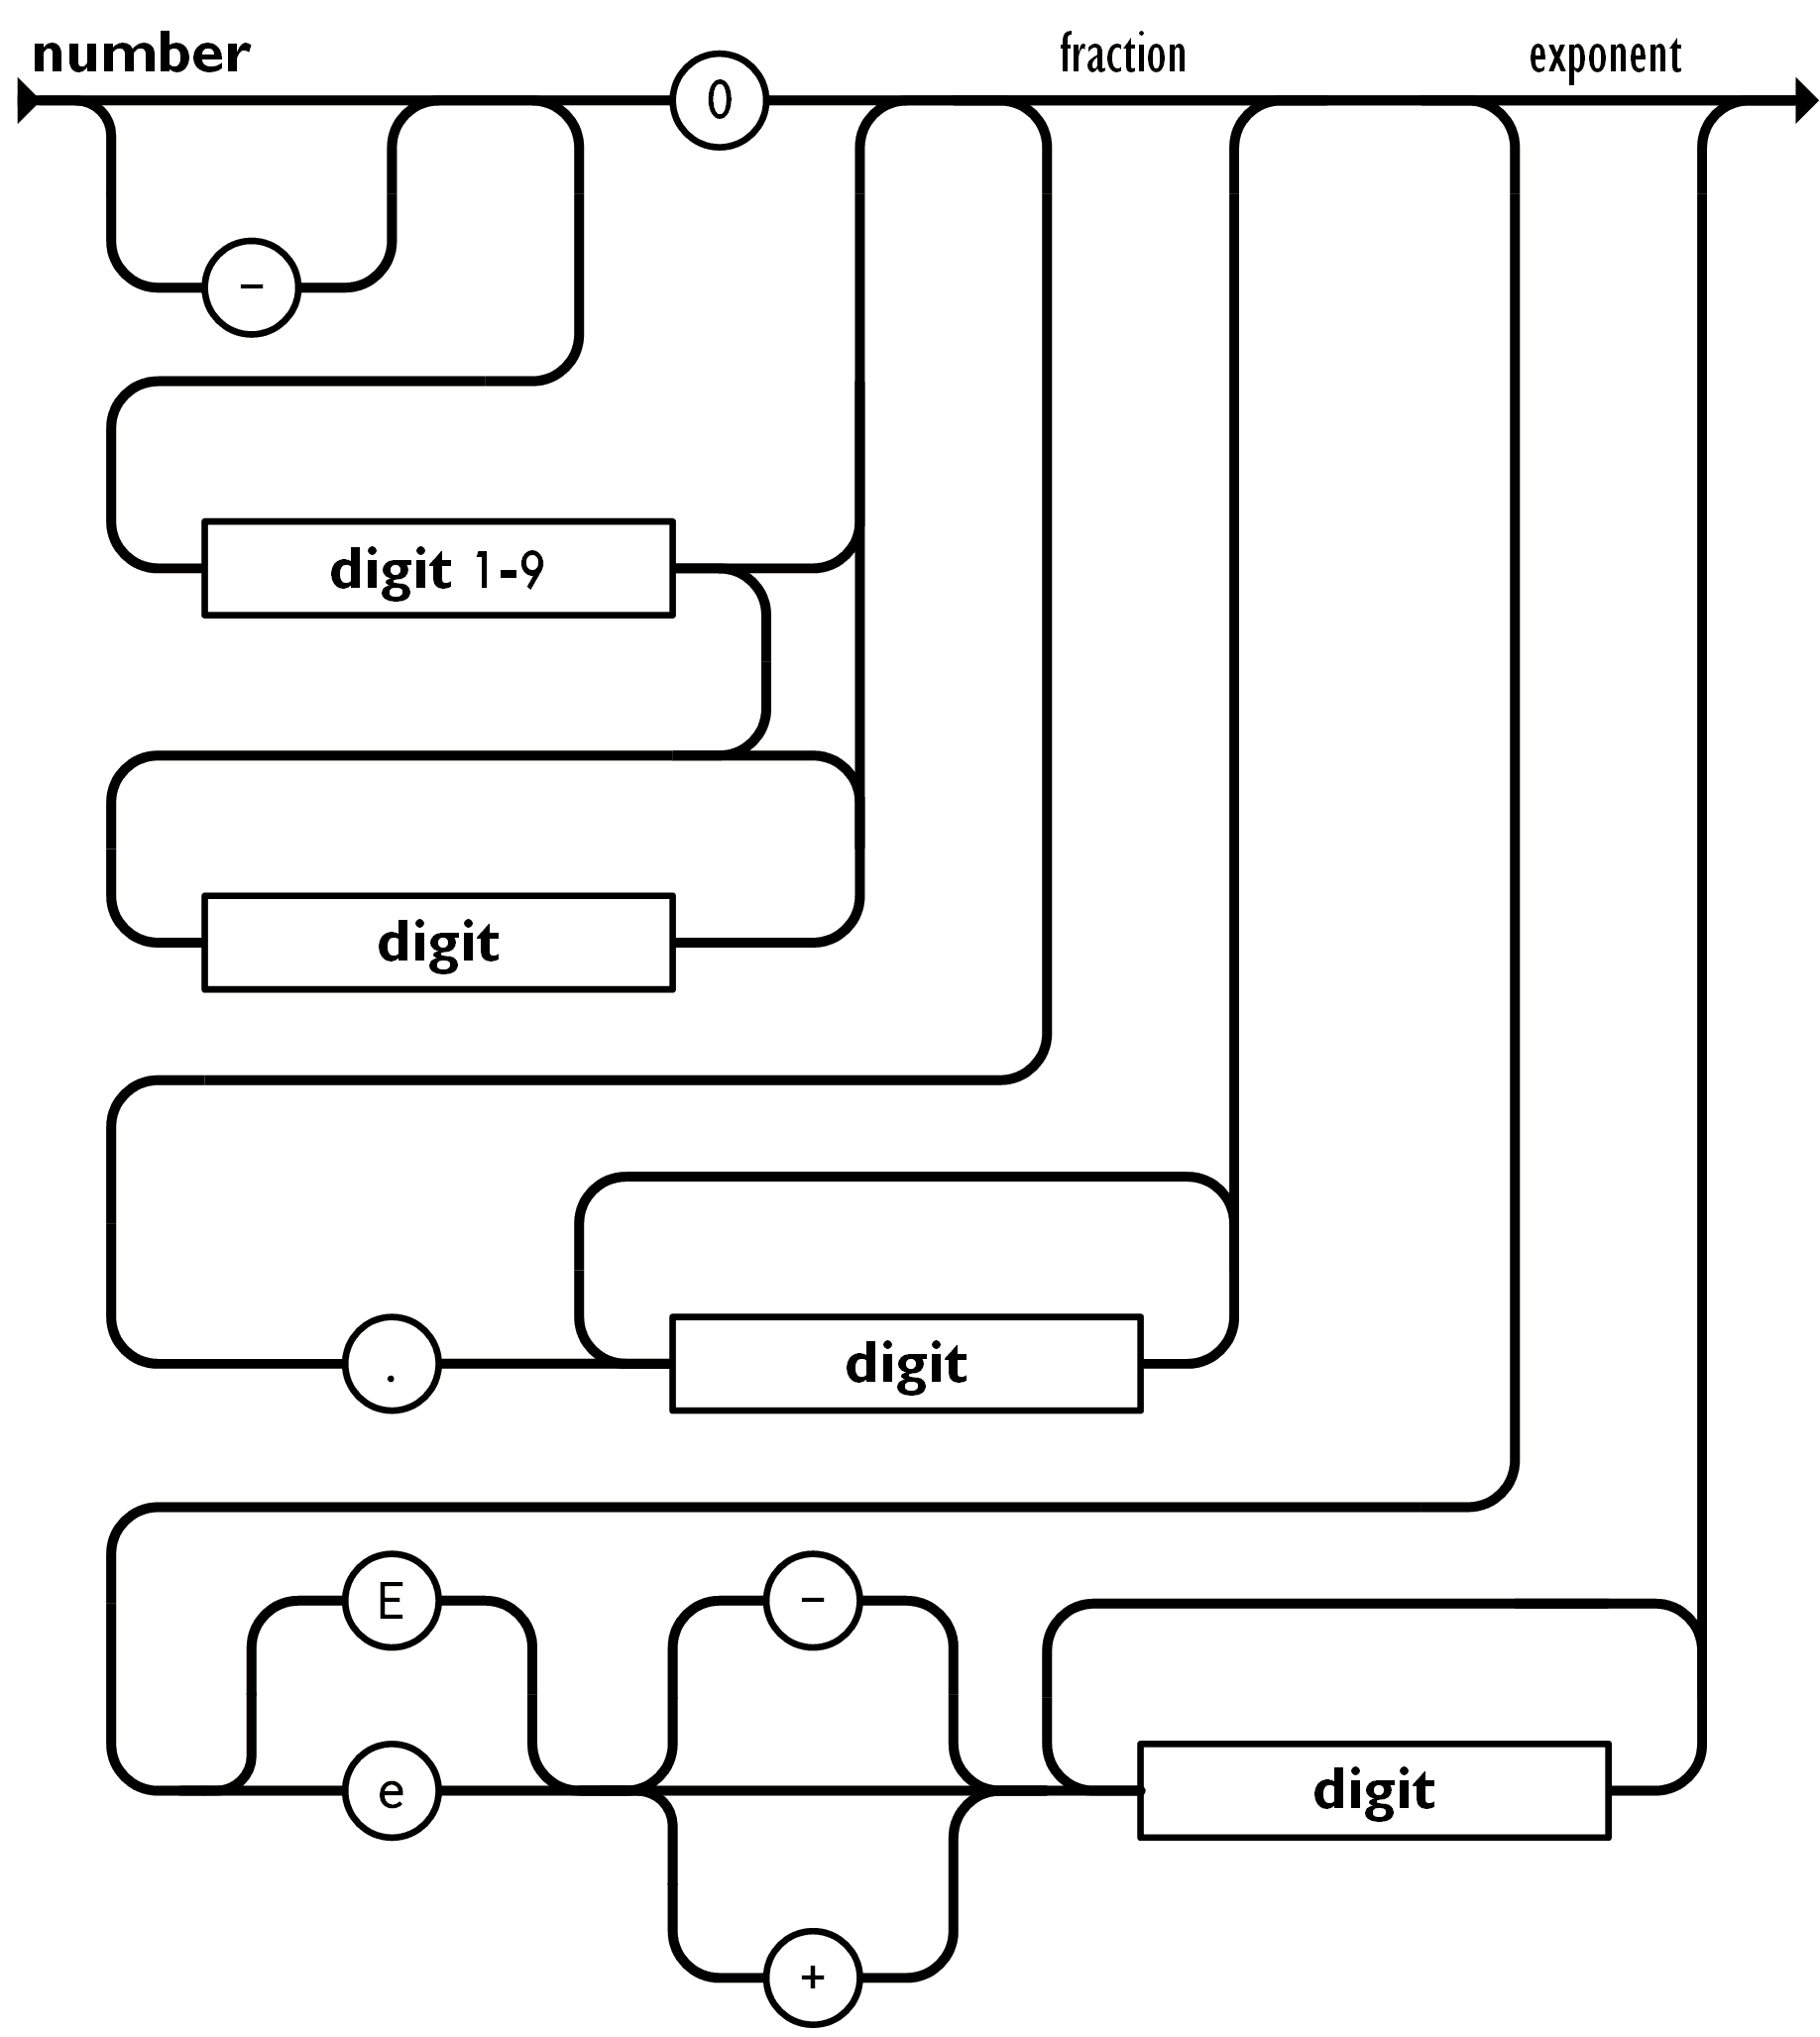
\includegraphics[scale=0.6]{number.png}
	\item Пробел \\
	      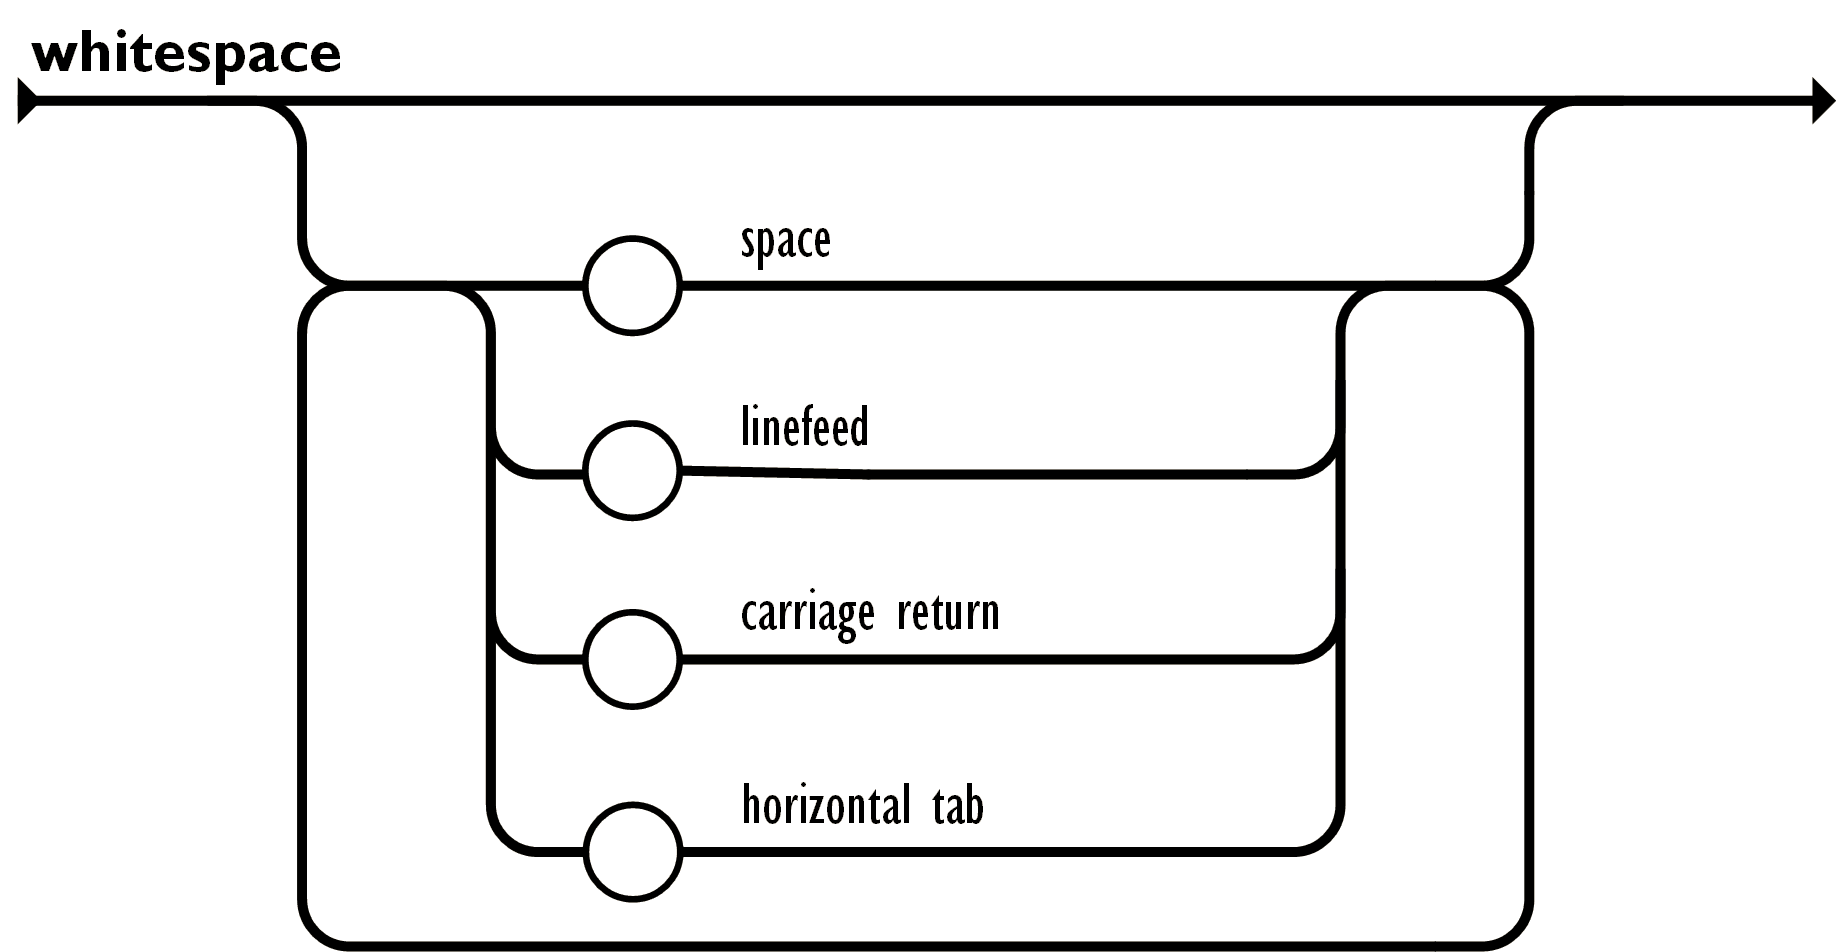
\includegraphics[scale=0.6]{whitespace.png}
\end{enumerate}

\newpage
\addcontentsline{toc}{section}{Список литературы}
\printbibliography
\end{document}
